\section{Simulations}

For all the simulations we set the physical parameters \(x_L = -1\), \(x_R = 1\), \(x_0 = -0.5\), \(\sigma_\textrm{norm} = 0.04\), \(n = 16\) and \(t_\textrm{fin} = 0.1\), unless specified otherwise. All physical values take arbitrary units as we imposed \(\hbar = 1\). We take \(n_x = 256\) mesh intervals and \(\Delta t = 10^{-4}\) for the numerical parameters, again unless specified otherwise.

\subsection{Infinite potential well}

In this section we will consider \(V_0 = 0\), which means that the particle is stuck in an infinite potential well as imposed by the border conditions. Let's first look at the propagation of a single particle and its properties.

The wave function, representing the probability distribution of finding the particle in a spatial interval, is shown in \autoref{fig:i_normpsi}. From this figure, we notice that the wave spreads out over time, and after hitting the potential wall gets reflected back. We observe an interesting phenomenon with this reflection: it seems that the wave gets reflected at different speeds, resulting in multiple peaks, slower waves remaining close to the wall before fading away and faster waves getting reflected to the other side.

\begin{figure}[h]
    \centering
    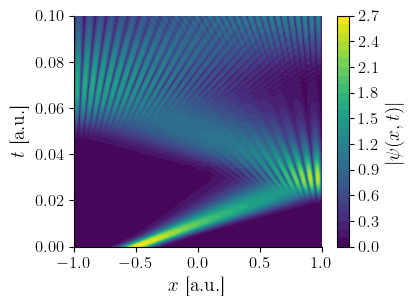
\includegraphics[width=0.6\linewidth]{figures/i_normpsi.png}
    \caption{Probability distribution of particle over space and time.}
    \label{fig:i_normpsi}
\end{figure}

Now that we've seen the general "motion" of the particle, let's analyse some of its properties. Firstly, its average position is shown in \autoref{fig:i_xmoy}. We can se it initially moves as we would expect a classical particle to move (which we will compare later). When it reaches the right hand side border, it gets reflected and the average position seems to move a bit slower than before the reflection, before regaining the same speed. On the second bounce however, the average position seems to stabilise a bit, which is coherent with what we saw before: the reflections seperate the wave function in multiple thinner parts. The average position then doesn't mean very much, with the position being multiple similarly sized peaks. \autoref{fig:i_pmoy} shows the average momentum of the particle. The momentum remains constant before the particle "collides" with the wall, which is also what was observed with the constant average position change on the previous figure. After the collision, the sign of the momentum flips around, meaning the wave is moving left. It is not an abrupt change, as would be expected from a wave. After a second reflection, the average momentum doesn't seem to reach the initial momentum again. This could be explained because of the spreading of the wave, where on average the wave moves slower than initially.

\begin{figure}[h]
    \centering
    \begin{subfigure}{0.48\linewidth}
        \centering
        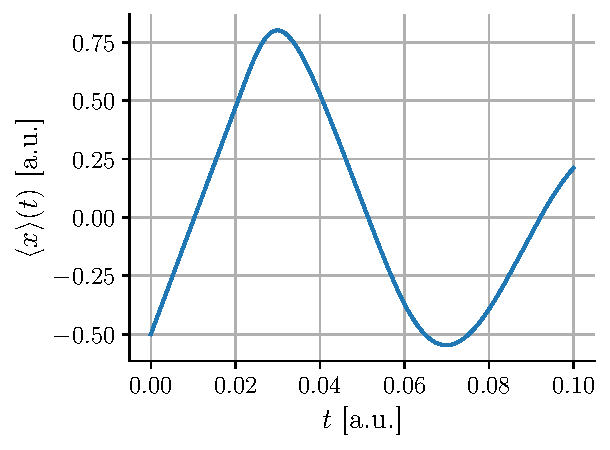
\includegraphics[width=\linewidth]{figures/i_xmoy.pdf}
        \caption{Average position}
        \label{fig:i_xmoy}
    \end{subfigure}
    \begin{subfigure}{0.48\linewidth}
        \centering
        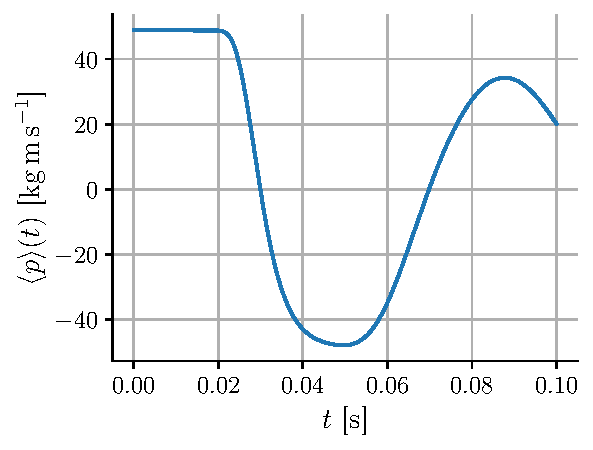
\includegraphics[width=\linewidth]{figures/i_pmoy.pdf}
        \caption{Average momentum}
        \label{fig:i_pmoy}
    \end{subfigure}
    \caption{Average position and momentum of a quantum particle in an infinite potential well}
    \label{fig:i_xmoy_pmoy}
\end{figure}

For a quantuum particle the uncertainty of its position and momentum is also a key property. 

\begin{figure}[h]
    \centering
    \begin{subfigure}{0.48\linewidth}
        \centering
        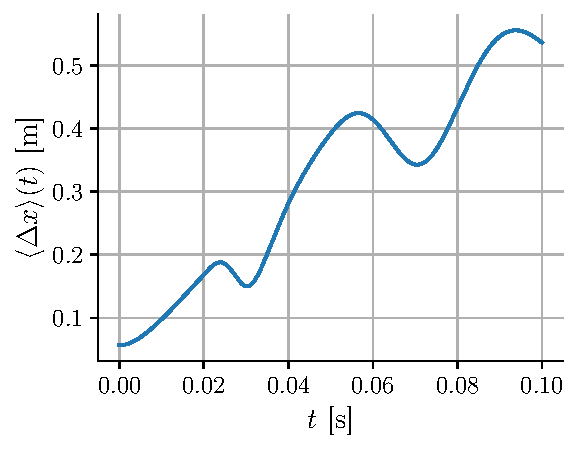
\includegraphics[width=\linewidth]{figures/i_deltax.pdf}
        \caption{Position spread}
        \label{fig:i_deltax}
    \end{subfigure}
    \begin{subfigure}{0.48\linewidth}
        \centering
        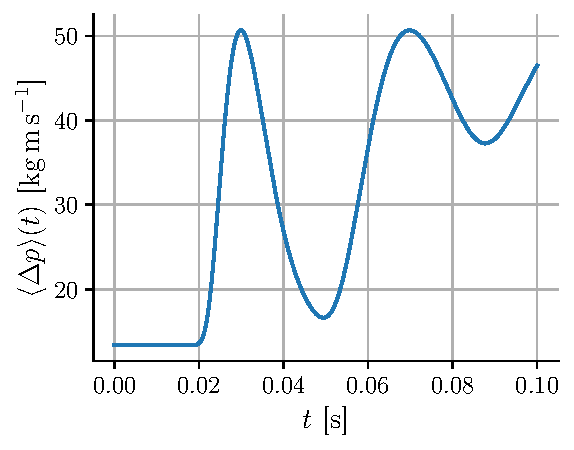
\includegraphics[width=\linewidth]{figures/i_deltap.pdf}
        \caption{Momentum spread}
        \label{fig:i_deltap}
    \end{subfigure}
    \caption{feur}
    \label{fig:i_deltax_deltap}
\end{figure}

\begin{figure}[h]
    \centering
    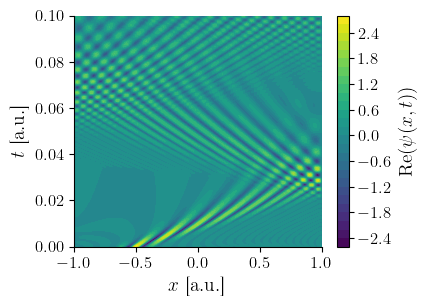
\includegraphics[width=0.6\linewidth]{figures/i_repsi.png}
    \caption{feur}
    \label{fig:i_repsi}
\end{figure}

\begin{figure}[h]
    \centering
    \begin{subfigure}{0.48\linewidth}
        \centering
        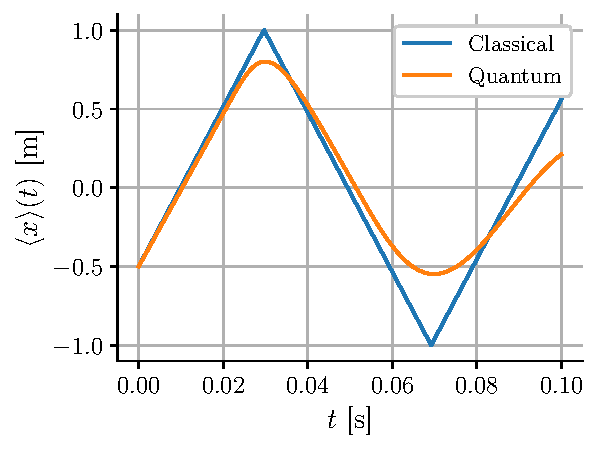
\includegraphics[width=\linewidth]{figures/i_classical_vs_quantum_energy.pdf}
        \caption{Same energy}
        \label{fig:i_classical_vs_quantum_energy}
    \end{subfigure}
    \begin{subfigure}{0.48\linewidth}
        \centering
        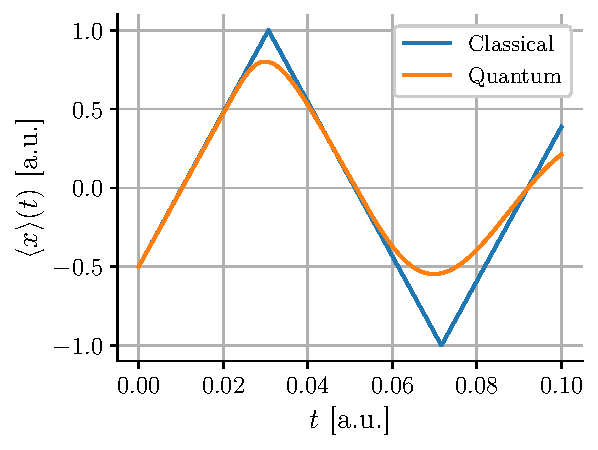
\includegraphics[width=\linewidth]{figures/i_classical_vs_quantum_momentum.pdf}
        \caption{Same initial momentum}
        \label{fig:i_classical_vs_quantum_momentum}
    \end{subfigure}
    \caption{feur}
    \label{fig:i_classical_vs_quantum}
\end{figure}

\begin{figure}[h]
    \centering
    \begin{subfigure}{0.55\linewidth}
        \centering
        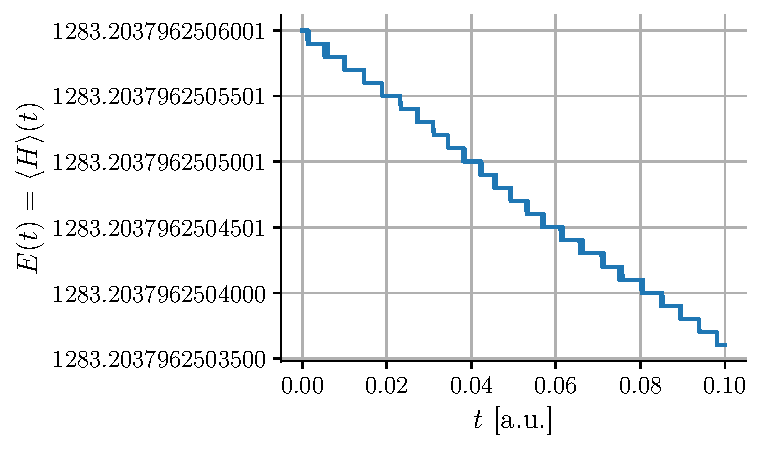
\includegraphics[width=\linewidth]{figures/i_conservation_energy.pdf}
        \caption{Energy of particle}
        \label{fig:i_conservation_energy}
    \end{subfigure}
    \begin{subfigure}{0.44\linewidth}
        \centering
        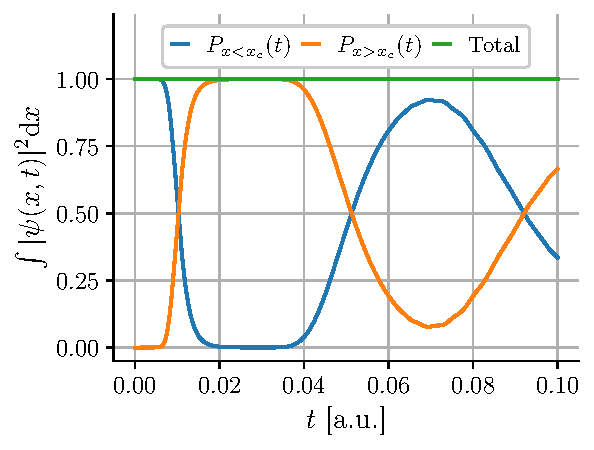
\includegraphics[width=\linewidth]{figures/i_conservation_probability.pdf}
        \caption{Normalisation}
        \label{fig:i_conservation_probability}
    \end{subfigure}
    \caption{Conservation of the particle's physical properties}
    \label{fig:i_conservation}
\end{figure}

\begin{figure}[h]
    \centering
    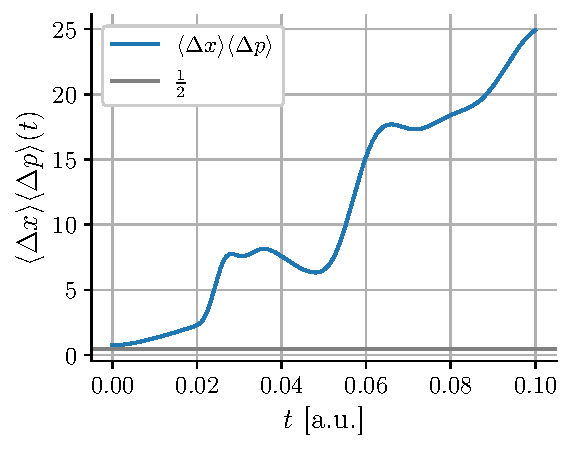
\includegraphics[width=0.6\linewidth]{figures/i_heisenberg.pdf}
    \caption{Verification of Heisenberg's uncertainty principle}
    \label{fig:i_heisenberg}
\end{figure}